
The model body of BERT has four main components, illustrated in Figure \ref{fig:bert-model-body-overview}.

\begin{figure}[H]
    \centering
    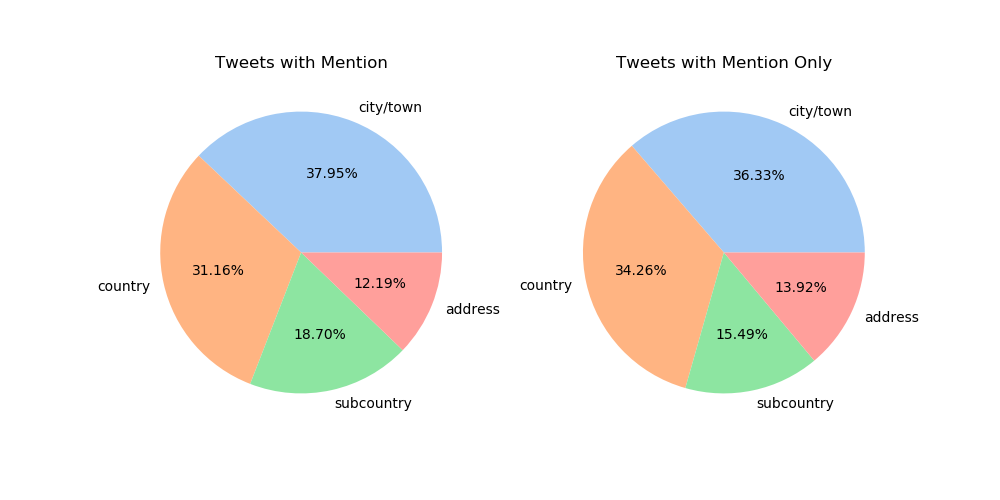
\includegraphics[width=0.5\textwidth]{images/mention_pie.png}
    \caption{BERT Model Body Structure}
    \label{fig:bert-model-body-overview}
\end{figure}

\begin{description}
   \item[Input Embeddings:] Input IDs obtained from the tokenization step are mapped to input embeddings using a lookup table (\cite{rohrer_transformers_2021}). These embeddings as starting points that are later adjusted to include more context (\cite{geron_hands-machine_2019}).
   
   \item[Positional Encoding:] The input embeddings do not contain information about where words are located in the input sentence. Positional encoding is added to the input sequence to fix this. (\cite{devlin_bert_2019})
   
   \item[Segment Embeddings:] \textcolor{red}{insert explanation}
   
   \item[Transformer Layers:] The token embeddings are then processed through multiple transformer layers, which use self-attention to capture the contextual relationships between tokens in the sequence. The transformer layers enable BERT to generate context-sensitive embeddings that capture the meaning of words based on their surrounding context. (\cite{devlin_bert_2019}) 
\end{description}

The output of the model body is an embedding vector for each token that captures its meaning in the context of the input sequence. \cite{tunstall_natural_2022}

Each of the above components is discussed in the subsequent sections.

Table \ref{tab:hyperparameters} shows the hyperparameters of BERT. 

\textcolor{red}{put hyperparameters in context and the table below as a summary}

\begin{table}[h]
\centering
\begin{tabular}{r|l}
\hline
    %\multicolumn{3}{c}{\textbf{Geotagged}} & \multicolumn{3}{c}{\textbf{Geotagged Only}} \\
    %\hline
    Hyper-parameter & Value \\
    \hline
     $d_\text{model}$ & $768$ \\
     $L$ & $12$ \\
     $A$ & $12$ \\
     $H$ & $768$ \\
     $d_\text{v}, d_\text{k}$ & $\frac{d_\text{model}}{A} = 64$ \\
     $d_{ff}$ & $4d_\text{model} = 3072$ \\
     \hline
\end{tabular}
\caption{BERT Base Body Hyperparameters \cite{devlin_bert_2019}}
\label{tab:hyperparameters}
\end{table}

%Now, onto discussing these components in proper, rigorous mathematical detail.